\documentclass{llncs}

\usepackage{llncsdoc}
\usepackage{graphicx,url}
\usepackage[brazil]{babel}
\usepackage[utf8]{inputenc}
\usepackage{float}
\usepackage{setspace}

\usepackage{tabularx}
\usepackage{cite}
\usepackage{hyperref}

\begin{document}
\sloppy
\title{Pushing Together: A platform for social participation}

\author{Tallys Martins\inst{2}, Dylan Guedes\inst{2},
        Luan Guimarães\inst{2}, Paulo Meirelles\inst{1,2}}

\institute{Instituto de Matemática e Estatística -- Universidade de São Paulo (USP)\\
  Rua do Matão, 1010 -- 05508-090 -- Cidade Universitária -- São Paulo -- SP -- Brasil\\
  \email{\{diegoamc,manzo\}@ime.usp.br}
  \and
  Faculdade do Gama -- Universidade de Brasília (UnB)\\
  Gama -- DF -- Brasil\\
  \email{\{tallysmartins,djmgguedes,livreluan\}@gmail.com, paulormm@unb.br}}

\maketitle
\begin{abstract}
  % Contexto
  The brazilian government, as many others around the world, has been trying to
  build technologies for social participation in a collaborative way, exploring
  the guidance of the internet.
  % Problema
  Still, the participation process is more than just giving your opinion, it is
  also about dialog and discussion in a way we should have clear vision about all sides,
  all points of view, all kind of opinions, to discuss what is the best solution
  to a problem. However, the social networks and the recommendation systems, in their
  current design make a barrier in a way that we only receive content about
  what we like, about what we follow, about what our friends like. We are 
  stuck in bubbles of opinion.
  % Soluções propostas
  With this work we present Pushing Together, a free software platform
  for collaborative participation with the aim of breaking the bubbles that
  freezes people in their mindsets. The goal is to identify diferent groups of
  opinion in a conversation using clustering algorithms, and then give power to some
  special actors, bringing interaction between the groups.
  % Frase de impacto
  Through this project we hope to increase the engagement of people in terms of
  social participation and provide new resources for democracy processes.

\textbf{Keywords:} social participation, bubbles of opinion, democracy, gamification
\end{abstract}


\section{Introduction}
\label{sec:intro}
  Em 2009 no Brasil, uma discussão sobre uma lei de regulamentação sobre a internet
  ficou internacionalmente conhecida pela sua relevância política bem como
  pelo formato aberto e colaborativo que foi adotado para a construção da lei.
  Uma consulta pública esteve aberta de outubro de 2009 a 30 de maio de 2010 e recebeu,
  nas suas duas fases, aproximadamente 2.000 comentários.
  No entanto, ainda que tenha sido inédita em construir uma legislação de forma tão aberta
  na rede, extrapolando o limite dos gabinetes e grupos organizados, vale apontar
  que a maioria dos comentários foram feitos por uma pequena parcela de participantes.
  Esse padrão de engajamento relativamente limitado se repetiu em outras consultas
  interativas realizadas. Percebemos que a participação oscila entre
  algumas dezenas ou centenas de pessoas e comentários, o que está longe do ideal de
  inclusão esperado pelo uso das tecnologias adotas, totalmente abertas e acessíveis.

  Promover a participação social é uma ação com muitos desafios que podem
  ser analisados em diferentes aspectos. Talvez o principal deles seja descobrir
  as melhores maneiras de deixar o processo no domínio  de pessoas leigas e 
  pessoas empoderadas mantendo o engajamento dos participantes. Esta estrutura
  de discussões em fórums/threads, não provê uma dinâmica atrativa para
  quem quer discutir. Além do mais, fica impraticável fazer análises mais aprofundadas,
  como por exemplo, identificar quais são os grupos de opinião formados, ou ainda
  que opinião é maioria ou minoria em uma dada consulta. Técnicas de análise
  de sentimento por processamento de linguagem natural não teriam eficácia
  dados os diferentes temas e contextos de cada conversas, e ainda diversos
  idiomas na rede.

  O projeto Pushing Together quer utilizar um novo conceito para os debates
  chamado aqui de participação crowdsourcing, que tem se mostrado uma ótima opção
  para quebrar as barreiras do engajamento a abrir mais espaço para o debate. Com
  pouco esforço, os participantes podem dar sua opinião apenas concordando
  e/ou discordando de opiniões já explicitadas por outros participantes, é algo
  como analisar os likes em um post do facebook.

  Desta maneira, ao facilitar a interação dos usuários na conversa, conseguimos
  aumentar a participação de usuários em x\%. Além disso, ao estruturar
  a opinião das pessoas em termos de concordo ou não concordo, 0 ou 1, é
  possível conseguir análises sofisticadas a respeito do que as pessoas
  pensam sobre a discussão. E é nessas análises que o pushing together quer atua,
  para permitir uma interação entre os diferentes grupos de opinião formados, dando
  poderes de push para atores especiais, pessoas com perfis considerados ativistas,
  mediadores e também os próprios 'donos' da consulta. Com o push, esses atores
  são capazes de gerar eventos e mensagens diretas, afetando a comunicação
  entre pessoas com diferentes opiniões. Com essa estratégia, pretendemos
  quebrar a barreira das bolhas de opinião formadas pela arquitetura
  atual da rede.

%Métricas de código-fonte estático são medidas extraídas a partir das análises
%léxica e sintática deste sem compilá-lo ou executá-lo e podem ser primitivas ou
%compostas, ou seja, formadas pela composição de uma ou mais métricas
%primitivas. Sua principal função é fornecer informações sobre complexidade,
%compreensão, testabilidade, manutenibilidade e evolução do
%código (REF).
%
%Exemplos de métricas podem ser simples como linhas de código e quantidade de
%métodos por classe ou complexas como conexões aferentes de uma classe.  Hoje
%existem diversas ferramentas para a simples extração de métricas como
%pylint\footnote{\url{http://www.pylint.org/}} (Python),
%metric\_fu\footnote{\url{https://github.com/metricfu/metric_fu}} (Ruby) e
%Analizo\footnote{\url{http://www.analizo.org/}} (C/C++ e Java), cada uma com
%diferentes graus de usabilidade, padrões e conjuntos de métricas, sendo
%necessária a criação de uma plataforma que reúna, organize e apresente essas
%informações ao usuário, em espcial, no controle da qualidade de um
%software durante sua evolução no tempo.
%
%As ferramentas de extração de métricas, em geral, não apresentam uma interface
%amigável para seres humanos lerem seus resultados e muito menos um padrão entre
%si.  Nesse contexto, este trabalho apresenta a plataforma Mezuro que
%(i) possui interface que agrupe as diversas ferramentas disponíveis;
%(ii) permita seleção e composição de métricas de forma flexível;
%(iii) mantém de um histórico de evolução;
%(iv) exibe os resultados de forma amigável;
%(v) permite ao usuário a criar seus parâmetros de interpretação conforme um
%contexto (por exemplo, linguagem de programação e domínio de aplicação).

\section{Related tools}

 Existe uma ferramenta que foi construida em cima do conceito de participação
 crowdsourcing e que serviu de inspiração no desenvolvimento do projeto Pushing
 Together. O Polis\footnote{\url{https://pol.is}} oferece aos usuários a possibilidade
 de criar uma discussão em que as pessoas fazem comentários de
 até 140 caracteres demonstrando seu ponto de vista. Os comentários então são
 apresentados como tópicos em cards. A interação na plataforma ocorre com outros
 usuários concordando ou discordando de um comentário existente ou ainda por
 adição de novos comentários à conversa.

 Representando os usuários como um vetores de 0 e 1 para as opções nas propostas
 é possível separar grupos opinião com técnicas de clusterização de dados.
 Com isto, o Polis apresenta vários insights sobre a discussão, entre eles, quais grupos de opinião formados, quais
 propostas mais votadas por grupo, quais são os grupos de maioria e minoria.

  \begin{figure}[H]
    \centering
      \begin{minipage}{.50\textwidth}
        \includegraphics[width=.9\linewidth]{images/polis1.png}
        \caption{Cards with comments}
        \label{fig:polis-2}
      \end{minipage}
      \begin{minipage}{.49\textwidth}
        \includegraphics[width=.9\linewidth]{images/polis2.png}
        \caption{Groups of opinion formed}
        \label{fig:polis-1}
      \end{minipage}
  \end{figure}

 A ideia inicial do projeto era contribuir e evoluir a ferramenta Polis, de maneira
 que fosse possível desenvolver a gamificação, suporte mobile e sistema de notificações.
 No entanto, a comunidade Polis não demonstrou tanta abertura e tivemos dificuldades
 em seguir essa abordagem por falta de documentação, transparência e suporte da
 comunidade criadora do software.

 Com as barreiras encontradas, decidimos criar o sistema com uma arquitetura independente do Polis,
 como uma capa, a um nível de abstração superior. Dessa maneira, caminhamos agora para consumir
 serviços de um módulo de clusterização próprio, nascido para ser transparente e com uma comunidade aberta.

\section{The Pushing Together project}
\label{sec:mezuro}

O Pushing Together nasceu em uma espécie de Hackaton. Uma
ideia da ONG brasileira Cidades Democráticas que participou do evento chamado Inteligência Coletiva
para a Democracia, na cidade de Madrid, na Espanha. O projeto é dividido em uma
aplicação front end escrita em React Native e um servidor NodeJS.

O módulo servidor é responsável por gerenciar os usuários e os
recursos de push da gamificação, fazendo também a interface com o módulo externo
de processamento dos clusters. Toda a comunicação, tanto da aplicação front end,
quanto com o módulo de clusterização é feita através de uma API.

Devido as limitações já apresentadas sobre a plataforma Polis, um novo módulo de
clusterização está sendo pensado para substituir a construção iniciada em cima
do Polis. A figura \ref{fig:architecture-2} abaixo descreve de maneira geral essa arquitetura.

\begin{figure}[H]
  \centering
    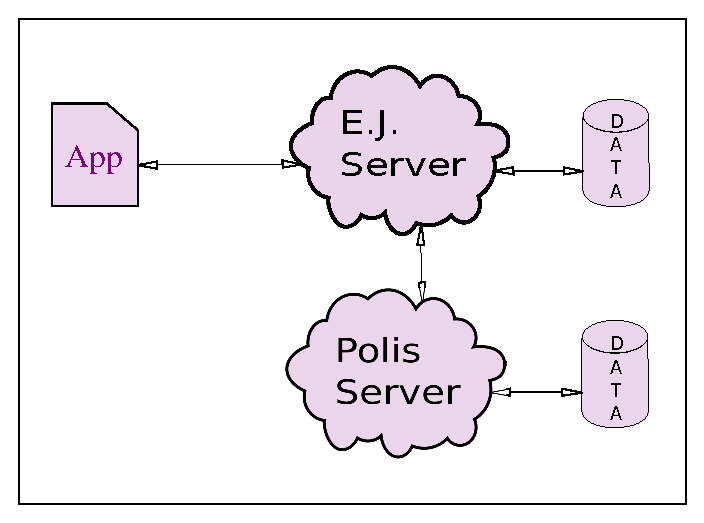
\includegraphics[keepaspectratio=true,,scale=0.6]{images/architecture-1.eps}
  \caption{Architecture of the system}
  \label{fig:architecture-2}
\end{figure}

No Pushing Together então foram pensados 3 tipos de perfis a serem identificad

\begin{itemize}
  \item Conversa
    \begin{itemize}
    \item \textit{Download} do código-fonte a partir de repositórios (Git, Subversion, Bazaar etc) ou via arquivo compactado;
        \item Escolha da periodicidade do processamento do código (1 dia, 2 dias, semanal, quinzenal e mensal);
        \item Escolha de qual configuração de métricas cada repositório irá utilizar;
        \item Nota de cada métrica da configuração para cada arquivo do repositório;
        \item Análise gráfica de cada arquivo do repositório por meio de um gráfico de pontos com notas ao longo do tempo;
        \item Resultados públicos e acessíveis à comunidade.
    \end{itemize}
    \item Configuração
    \begin{itemize}
    \item Criação de configuração e a possibilidade de clonagem;
        \item Estatísticas sobre as configurações mais populares dentro da comunidade;
        \item Criação de intervalos qualitativos associados aos valores das métricas;
        \item Criação de grupos de leitura para a interpretação textual dos resultados das métricas;
        \item Combinações de métricas nativas para criação de análises compostas e mais complexas.
    \end{itemize}
\end{itemize}

O Mezuro tem o formato de uma rede social, no qual os participantes podem ver a
produção de terceiros por meio da avaliação dos projetos ou do clone das
configurações. Essa interação mútua e aberta pode ser interessante para
desenvolvedores, gerentes de projeto, auditores de software e até
mesmo uma equipe de desenvolvimento inteira. O objetivo final é criar uma
comunidade que veja o valor de tais metodologias e como isso pode contribuir
para o sucesso do seu projeto.

\section{Final remarks}

O Mezuro surge como uma potencial resposta para a falta de monitoramento e
padronização de código-fonte e a necessidade de avaliação do mesmo,
considerando que é um \textit{software} livre, altamente customizável, com
suporte para muitas linguagens computacionais, interface amigável, que fornece
histórico de processamentos e também com uma arquitetura planejada para
incorporar novas funcionalidades.

%TODO Paulo: mais coisas ...

\bibliographystyle{splncs03}
\bibliography{mezuro}
\end{document}
